\documentclass[12pt]{article}
\usepackage[paper=letterpaper,margin=2cm]{geometry}
\usepackage{amsmath}
\usepackage{amssymb}
\usepackage{amsfonts}
\usepackage{newtxtext, newtxmath}
\usepackage{enumitem}
\usepackage{titling}
\usepackage{svg}
\usepackage{xcolor}
\usepackage{listings}
\usepackage{float}
\usepackage{multicol}
\usepackage{nicefrac}
\usepackage[colorlinks=true]{hyperref}

\setlength{\droptitle}{-6em}

\definecolor{codegreen}{rgb}{0,0.6,0}
\definecolor{codegray}{rgb}{0.5,0.5,0.5}
\definecolor{codepurple}{rgb}{0.58,0,0.82}
\definecolor{backcolour}{rgb}{0.95,0.95,0.92}

\lstdefinestyle{mystyle}{
    commentstyle=\color{codegreen},
    keywordstyle=\color{magenta},
    numberstyle=\tiny\color{codegray},
    stringstyle=\color{codepurple},
    basicstyle=\ttfamily\footnotesize,
    breakatwhitespace=false,
    breaklines=true,
    captionpos=b,
    keepspaces=true,
    numbers=left,
    numbersep=5pt,
    showspaces=false,
    showstringspaces=false,
    showtabs=false,
    tabsize=2
}

\lstset{
        style=mystyle,
        inputencoding=utf8,
        extendedchars=true,
}


\title{\large{Aprendizagem 2022}\vskip 0.2cm Homework II -- Group 019\vskip 0.2cm Diogo Gaspar 99207, Rafael Oliveira 99311}
\date{}
\begin{document}
\maketitle
\center\large{\vskip -2.5cm\textbf{Part I}: Pen and paper}
\begin{enumerate}[leftmargin=\labelsep]

  \item \textbf{Compute the recall of a distance-weighted $k$NN with $k=5$ and distance
  $d(x_1, x_2) = \operatorname{Hamming(x_1, x_2)} + \frac{1}{2}$ using leave-one-out
  evaluation schema (i.e., when classifying one observation, use all remaining ones).}

  For starters, it's worth noting that, in this context, the \textbf{Hamming distance} between two
  observations $x_1$ and $x_2$ is defined as the number of attributes that differ between them.

  Knowing this, we can now create an $8 \times 8$ matrix (as can be seen below), where each entry
  represents the Hamming distance ($+ \frac{1}{2}$) between two observations. This matrix is symmetric, of course.
  Each column $i$, here, will have $8 - 1 = 7$ associated entries, each representing the distance $d$
  between the observation $x_i$ and the remaining $7$ observations: we will, then,
  pick the $k = 5$ nearest neighbors according to said distance, classifying $x_i$
  in a \textbf{distance-weighted} manner.

  \begin{table}[h]
    \setlength{\tabcolsep}{5pt} % column spacing
    \renewcommand{\arraystretch}{1.35} % row spacing
    \centering
    \label{tab:my-table}
    \begin{tabular}{lllllllll}
          & $x_1$                           & $x_2$                           & $x_3$                           & $x_4$                           & $x_5$                           & $x_6$                           & $x_7$                           & $x_8$                           \\
    $x_1$ & $\times$                        & $\nicefrac{5}{2}$                   & $\textcolor{teal}{\nicefrac{3}{2}}$ & $\textcolor{teal}{\nicefrac{1}{2}}$ & $\textcolor{teal}{\nicefrac{3}{2}}$ & $\textcolor{teal}{\nicefrac{3}{2}}$ & $\textcolor{teal}{\nicefrac{3}{2}}$ & $\nicefrac{5}{2}$                   \\
    $x_2$ & $\nicefrac{5}{2}$                   & $\times$                        & $\textcolor{teal}{\nicefrac{3}{2}}$ & $\nicefrac{5}{2}$                   & $\textcolor{teal}{\nicefrac{3}{2}}$ & $\textcolor{teal}{\nicefrac{3}{2}}$ & $\textcolor{teal}{\nicefrac{3}{2}}$ & $\textcolor{teal}{\nicefrac{1}{2}}$ \\
    $x_3$ & $\textcolor{teal}{\nicefrac{3}{2}}$ & $\textcolor{teal}{\nicefrac{3}{2}}$ & $\times$                        & $\textcolor{teal}{\nicefrac{3}{2}}$ & $\nicefrac{5}{2}$                   & $\nicefrac{5}{2}$                   & $\textcolor{teal}{\nicefrac{1}{2}}$ & $\textcolor{teal}{\nicefrac{3}{2}}$ \\
    $x_4$ & $\textcolor{teal}{\nicefrac{1}{2}}$ & $\nicefrac{5}{2}$                   & $\textcolor{teal}{\nicefrac{3}{2}}$ & $\times$                        & $\textcolor{teal}{\nicefrac{3}{2}}$ & $\textcolor{teal}{\nicefrac{3}{2}}$ & $\textcolor{teal}{\nicefrac{3}{2}}$ & $\nicefrac{5}{2}$                   \\
    $x_5$ & $\textcolor{teal}{\nicefrac{3}{2}}$ & $\textcolor{teal}{\nicefrac{3}{2}}$ & $\nicefrac{5}{2}$                   & $\textcolor{teal}{\nicefrac{3}{2}}$ & $\times$                        & $\textcolor{teal}{\nicefrac{1}{2}}$ & $\nicefrac{5}{2}$                   & $\textcolor{teal}{\nicefrac{3}{2}}$ \\
    $x_6$ & $\textcolor{teal}{\nicefrac{3}{2}}$ & $\textcolor{teal}{\nicefrac{3}{2}}$ & $\nicefrac{5}{2}$                   & $\textcolor{teal}{\nicefrac{3}{2}}$ & $\textcolor{teal}{\nicefrac{1}{2}}$ & $\times$                        & $\nicefrac{5}{2}$                   & $\textcolor{teal}{\nicefrac{3}{2}}$ \\
    $x_7$ & $\textcolor{teal}{\nicefrac{3}{2}}$ & $\textcolor{teal}{\nicefrac{3}{2}}$ & $\textcolor{teal}{\nicefrac{1}{2}}$ & $\textcolor{teal}{\nicefrac{3}{2}}$ & $\nicefrac{5}{2}$                   & $\nicefrac{5}{2}$                   & $\times$                        & $\textcolor{teal}{\nicefrac{3}{2}}$ \\
    $x_8$ & $\nicefrac{5}{2}$                   & $\textcolor{teal}{\nicefrac{1}{2}}$ & $\textcolor{teal}{\nicefrac{3}{2}}$ & $\nicefrac{5}{2}$                   & $\textcolor{teal}{\nicefrac{3}{2}}$ & $\textcolor{teal}{\nicefrac{3}{2}}$ & $\textcolor{teal}{\nicefrac{3}{2}}$ & $\times$                       
    \end{tabular}
    \caption{Distance $d$ between observations - in teal, a given observation's $k$ nearest neighbors}
  \end{table}

  For each observation $x_i$, the $k$ nearest neighbors are, therefore, the ones represented in
  teal in the table above. Instead of predicting a class given the neighbors' mode,
  we'll want to choose it in a distance-weighted manner here: this means that, for each
  observation $x_i$, we'll want to compute the \textbf{weighted majority vote} of its $k$ nearest
  neighbors, where the weight of each neighbor is given by:

  $$w_{i, j} = \frac{1}{d(x_i, x_j)}$$

  where $x_j$ is one of the $k$ nearest neighbors of $x_i$. Considering the data gathered up until now,
  we'll have the following conclusions regarding the model's classification for each instance:

\begin{table}[h]
  \centering
  \renewcommand{\arraystretch}{1.35} % row spacing
  \begin{tabular}{c|c|c|c}
        & Weighted distance to $N$                                & Weighted distance to $P$                                & Predicted Class \\
  $x_1$ & $3 * \nicefrac{1}{(\nicefrac{3}{2})} = \textcolor{purple}{2}$                           & $ \nicefrac{1}{(\nicefrac{3}{2})} + \nicefrac{1}{(\nicefrac{1}{2})} = \textcolor{teal}{\nicefrac{8}{3}}$    &  $P$               \\
  $x_2$ & $3 * \nicefrac{1}{(\nicefrac{3}{2})} + \nicefrac{1}{(\nicefrac{1}{2})} = \textcolor{teal}{4}$ & $ \nicefrac{1}{(\nicefrac{3}{2})} = \textcolor{purple}{\nicefrac{2}{3}}$                              &  $N$               \\
  $x_3$ & $ \nicefrac{1}{(\nicefrac{3}{2})} + \nicefrac{1}{(\nicefrac{1}{2})} = \textcolor{teal}{\nicefrac{8}{3}}$    & $3 * \nicefrac{1}{(\nicefrac{3}{2})} = \textcolor{purple}{2}$                           &  $N$               \\
  $x_4$ & $3 * \nicefrac{1}{(\nicefrac{3}{2})} = \textcolor{purple}{2}$                           & $ \nicefrac{1}{(\nicefrac{3}{2})} + \nicefrac{1}{(\nicefrac{1}{2})} = \textcolor{teal}{\nicefrac{8}{3}}$    &  $P$               \\
  $x_5$ & $ \nicefrac{1}{(\nicefrac{3}{2})} + \nicefrac{1}{(\nicefrac{1}{2})} = \textcolor{teal}{\nicefrac{8}{3}}$    & $3 * \nicefrac{1}{(\nicefrac{3}{2})} = \textcolor{purple}{2}$                           &  $N$               \\
  $x_6$ & $ \nicefrac{1}{(\nicefrac{3}{2})} + \nicefrac{1}{(\nicefrac{1}{2})} = \textcolor{teal}{\nicefrac{8}{3}}$    & $3 * \nicefrac{1}{(\nicefrac{3}{2})} = \textcolor{purple}{2}$                           &  $N$               \\
  $x_7$ & $2 * \nicefrac{1}{(\nicefrac{3}{2})} = \textcolor{purple}{\nicefrac{1}{3}}$                           & $3 * \nicefrac{1}{(\nicefrac{3}{2})} + \nicefrac{1}{(\nicefrac{1}{2})} = \textcolor{teal}{4}$ &  $P$               \\
  $x_8$ & $3 * \nicefrac{1}{(\nicefrac{3}{2})} = \textcolor{purple}{2}$                           & $ \nicefrac{1}{(\nicefrac{3}{2})} + \nicefrac{1}{(\nicefrac{1}{2})} = \textcolor{teal}{\nicefrac{8}{3}}$    &  $P$              
  \end{tabular}
  \caption{Distance weighting for each observation}
  \label{tab:my-table-1}
  \end{table}
  
  We'll have, given the data gathered above, the following confusion matrix:

  \begin{figure}[H]
    \centering
    \includesvg{../assets/hw2-1.1.svg}
    \caption{Confusion Matrix}
  \end{figure}

  Moreover, the \textbf{recall} of a classifier is defined as the ratio between the number of
  true positives and the number of true positives plus the number of false negatives that the
  classifier makes. Looking at the confusion matrix above, we can assert that the associated
  recall will, therefore, be:

  $$
  \frac{TP}{TP + FN} = \frac{2}{2 + 2} = \frac{2}{4} = 0.5
  $$

  \pagebreak

  \item \textbf{Considering the nine training observations, learn a Bayesian classifier assuming:
  i) $y_1$ and $y_2$ are dependent, ii) $\{y_1 , y_2\}$ and $\{y_3 \}$ variable sets are
  independent and equally important, and iii) $y_3$ is normally distributed. Show all parameters.}

  Considering both variable sets, $\{y_1, y_2\}$ and $\{y_3\}$, to be independent and equally important,
  it'll make sense to train a Naive Bayes classifier here, such that (and utilizing
  Bayes' theorem):

  $$
  P(C = ^N_P | y_1, y_2, y_3) = \frac{P(y_1, y_2, y_3 | C = ^N_P) P(C = ^N_P)}{P(y_1, y_2, y_3)}
  $$

  More so, since $\{y_1, y_2\}$ and $\{y_3\}$ are independent (and $y_1$ and $y_2$ are dependent),
  we can rewrite the above as:

  $$
  P(C = ^N_P | y_1, y_2, y_3) = \frac{P(y_1, y_2 | C = ^N_P) P(y_3 | C = ^N_P) P(C = ^N_P)}{P(y_1, y_2) P(y_3)}
  $$

  According to the Naive Bayes' assumption, "the presence (or absence) of a particular feature
  in a class is unrelated to the presence (or absence) of any other feature", so we will, in fact,
  only need the above equation's numerator to be able to classify a new observation.
  The goal here is to find:

  $$
  \operatorname{argmax}_{c \in \{N, P\}} P(y_1, y_2 | C = c) P(y_3 | C = c) P(C = c)
  $$

  For starters, we can note that, from the given training set:
  
  $$
  P(C = P) = \frac{5}{9}, \quad P(C = N) = \frac{4}{9}
  $$

  We also know that $y_3$ is normally distributed, meaning we'll have:

  $$
  P(y_3 | C = ^N_P) \sim \mathcal{N}(x | \mu, \sigma^2) = \frac{1}{\sqrt{2 \pi \sigma^2}} \exp \left( - \frac{(x - \mu)^2}{2 \sigma^2} \right)
  $$

  By also looking at the given training set (which includes the new, ninth sample), we'll be able
  to extrapolate the following probabilities:

  \pagebreak

  \begin{multicols}{2}
    \setlength{\columnseprule}{1pt}
    \def\columnseprulecolor{\color{black}}
    \centering
    $\textcolor{purple}{C = N}: P(\textcolor{purple}{C = N}) = \frac{4}{9}$
    \begin{itemize}
      \item $P(y_2 = A, y_2 = 0 | \textcolor{purple}{C = N}) = 0$
      \item $P(y_2 = A, y_2 = 1 | \textcolor{purple}{C = N}) = \frac{1}{4}$
      \item $P(y_1 = B, y_2 = 0 | \textcolor{purple}{C = N}) = \frac{2}{4} = \frac{1}{2}$
      \item $P(y_1 = B, y_2 = 1 | \textcolor{purple}{C = N}) = \frac{1}{4}$
    \end{itemize}
    Regarding $y_3$ and $\textcolor{purple}{N}$ labeled observations, we'll have the following parameters:
    
    $$
    \mu = \frac{1 + 0.9 + 1.2 + 0.8}{4} = 0.975
    $$
    $$
    \sigma^2 = \frac{1}{4 - 1} \sum_{i = 1}^4 (y_{3, i} - \mu)^2 = 0.029
    $$

    \columnbreak
    $\textcolor{teal}{C = P}: P(\textcolor{teal}{C = P}) = \frac{5}{9}$
    \begin{itemize}
      \item $P(y_1 = A, y_2 = 0 | \textcolor{teal}{C = P}) = \frac{2}{5}$
      \item $P(y_2 = A, y_2 = 1 | \textcolor{teal}{C = P}) = \frac{1}{5}$
      \item $P(y_1 = B, y_2 = 0 | \textcolor{teal}{C = P}) = \frac{1}{5}$
      \item $P(y_1 = B, y_2 = 1 | \textcolor{teal}{C = P}) = \frac{1}{5}$
    \end{itemize}
    Regarding $y_3$ and $\textcolor{teal}{P}$ labeled observations, we'll have the following parameters:

    $$
    \mu = \frac{1.2 + 0.8 + 0.5 + 0.9 + 0.8}{5} = 0.84
    $$
    $$
    \sigma^2 = \frac{1}{5 - 1} \sum_{i = 1}^5 (y_{3, i} - \mu)^2 = 0.063
    $$

  \end{multicols}

  The model is now ready to be used to classify new observations. Applying the model to
  the nine training observations, we'll have the following results:

  \begin{table}[h]
    \centering
    \renewcommand{\arraystretch}{1.35} % row spacing
    \resizebox{\columnwidth}{!}{%
    \begin{tabular}{c|c|c|c|c|c|c|c|c}
        & $y_1$ & $y_2$ & $y_3$ & Class & $P(\textcolor{purple}{C = N}) P(y_1, y_2, y_3 \mid \textcolor{purple}{C = N})$ & $P(\textcolor{teal}{C = P}) P(y_1, y_2, y_3 \mid \textcolor{teal}{C = P})$ & Predicted Class & Veredict \\
      $x_1$ & $A$   & $0$   & $1.2$ & $P$   & $0$                                    & $\frac{5}{9} \times \frac{2}{5} \times 0.92425$      & $P$             & $TP$     \\
      $x_2$ & $B$   & $1$   & $0.8$ & $P$   & $\frac{4}{9} \times \frac{1}{4} \times 0.15206$      & $\frac{5}{9} \times \frac{1}{5} \times 0.43669$      & $P$             & $TP$     \\
      $x_3$ & $A$   & $1$   & $0.5$ & $P$   & $\frac{4}{9} \times \frac{1}{4} \times 0.00264$      & $\frac{5}{9} \times \frac{1}{5} \times 0.08777$      & $N$             & $FN$     \\
      $x_4$ & $A$   & $0$   & $0.9$ & $P$   & $0$                                    & $\frac{5}{9} \times \frac{2}{5} \times 0.59446$      & $P$             & $TP$     \\
      $x_5$ & $B$   & $0$   & $1$   & $N$   & $\frac{4}{9} \times \frac{1}{2} \times 0.55836$      & $\frac{5}{9} \times \frac{1}{5} \times 0.73809$      & $N$             & $TN$     \\
      $x_6$ & $A$   & $0$   & $0.9$ & $N$   & $\frac{4}{9} \times \frac{1}{2} \times 0.32981$      & $\frac{5}{9} \times \frac{1}{5} \times 0.59446$      & $N$             & $TN$     \\
      $x_7$ & $B$   & $1$   & $1.2$ & $N$   & $\frac{4}{9} \times \frac{1}{4} \times 0.9068$       & $\frac{5}{9} \times \frac{1}{5} \times 0.92425$      & $P$             & $FP$     \\
      $x_8$ & $B$   & $1$   & $0.8$ & $N$   & $\frac{4}{9} \times \frac{1}{4} \times 0.15206$      & $\frac{5}{9} \times \frac{1}{5} \times 0.43669$      & $P$             & $FP$     \\
      $x_9$ & $B$   & $0$   & $0.8$ & $P$   & $\frac{4}{9} \times \frac{1}{2} \times 0.15206$      & $\frac{5}{9} \times \frac{1}{5} \times 0.43669$      & $P$             & $FP$    
    \end{tabular}%
    }
    \caption{Classification vs Real results}
    \label{tab:my-table-2}
  \end{table}

  \pagebreak

  \item \textbf{Under a MAP assumption, compute $P(Positive | x)$ of each testing observation.}

  Considering Bayes' theorem, we know $P(Positive | x)$ can also be written as follows:

  $$
  P(Positive | x) = \frac{P(x| Positive) P(Positive)}{P(x)}
  $$

  Since $x$ has two independent variable sets, $\{y_1, y_2\}$ and $\{y_3\}$, we'll be
  able to write the above expression as follows (note that $x$'s $y_1$ value will
  be written as $y_1$, and so on, for simplicity's sake):

  $$
  P(Positive | x) = \frac{P(y_1, y_2| Positive) P(y_3| Positive) P(Positive)}{P(y_1, y_2) P(y_3)}
  $$

  Let's consider the three samples given in the question's statement:

  $$
    x_1' = \begin{pmatrix}
      A \\
      1 \\
      0.8
    \end{pmatrix}, \quad
    x_2' = \begin{pmatrix}
      B \\
      1 \\
      1
    \end{pmatrix}, \quad
    x_3' = \begin{pmatrix}
      B \\
      0 \\
      0.9
    \end{pmatrix}
  $$

  Considering the training observations, we can gather that there are:

  \begin{multicols}{3}
    \setlength{\columnseprule}{1pt}
    \def\columnseprulecolor{\color{black}}
    \centering

    $x_1'$

    Among all (five) positive training samples, one with features $y_1 = A, y_2 = 1$,
    two with feature $y_3 = 0.8$.
    Among all (nine) training samples, two with features $y_1 = A, y_2 = 1$, three
    with feature $y_3 = 0.8$.

    \columnbreak

    $x_2'$

    Among all (five) positive training samples, one with features $y_1 = B, y_2 = 1$,
    zero with feature $y_3 = 1$.
    Among all (nine) training samples, two with features $y_1 = B, y_2 = 1$, one
    with feature $y_3 = 1$.

    \columnbreak

    $x_3'$

    Among all (five) positive training samples, one with features $y_1 = B, y_2 = 0$,
    one with feature $y_3 = 0.9$.
    Among all (nine) training samples, three with features $y_1 = B, y_2 = 0$,
    two with feature $y_3 = 0.9$.

  \end{multicols}

  Note, of course, that the probabilities regarding $y_1$ and $y_2$ features may
  be calculated in a discrete manner, directly utilizing the values gathered above.
  The same can't be said for $y_3$ with it being normally distributed:
  we'll need to calculate the parameters for it (note that Positive parameters were computed in the
  previous question), and only then will we be able to calculate the needed probabilities regarding
  these samples' $y_3$ values:

  \begin{align}
    \mu_{y_3, Positive} = 0.84, \quad \mu_{y_3, All} = \frac{(1.2 + 0.8 + \cdots + 0.8)}{9} = 0.9 \\
    \sigma_{y_3, Positive}^2 = 0.063, \quad \sigma_{y_3, All}^2 = \frac{1}{9 - 1} \sum_{i=1}^{9} (y_{3, i} - \mu)^2 = 0.0475
  \end{align}

  \begin{multicols}{3}
    \setlength{\columnseprule}{1pt}
    \def\columnseprulecolor{\color{black}}
    \centering

    $x_1'$

    $$
    \begin{aligned}
      &P(y_3 = 0.8 | P) = 0.43669, \\
      &P(y_3 = 0.8) = 0.32314
    \end{aligned}
    $$

    \columnbreak

    $x_2'$

    $$
    \begin{aligned}
      &P(y_3 = 1 | P) = 0.73809, \\
      &P(y_3 = 1) = 0.67686
    \end{aligned}
    $$

    \columnbreak

    $x_3'$

    $$
    \begin{aligned}
      &P(y_3 = 0.9 | P) = 0.59446, \\
      &P(y_3 = 0.9) = 0.5
    \end{aligned}
    $$

  \end{multicols}

  We can, therefore, assert that:

  \begin{align*}
    P(Positive | x_1') &= \frac{\nicefrac{1}{5} \times 0.43669 \times \nicefrac{5}{9}}{\nicefrac{2}{9} \times 0.32314} = 0.6756978 \\
    P(Positive | x_2') &= \frac{\nicefrac{1}{5} \times 0.73809 \times \nicefrac{5}{9}}{\nicefrac{2}{9} \times 0.67686} = 0.5452309 \\
    P(Positive | x_3') &= \frac{\nicefrac{1}{5} \times 0.59446 \times \nicefrac{5}{9}}{\nicefrac{3}{9} \times 0.5} = 0.3963067
  \end{align*}

  \pagebreak

  \item \textbf{Given a binary class variable, the default decision threshold of $\theta = 0.5$,
    $$
    f(x | \theta) = \begin{cases}
      Positive & \text{if } P(positive | x) > \theta \\
      Negative & otherwise
    \end{cases}
    $$
    can be adjusted. Which decision threshold – 0.3, 0.5 or 0.7 – optimizes testing accuracy?
  }

  As given by the question's statement, we know the actual class values of the testing observations.
  Moreover, we've calculated $P(Positive | x)$ for each of them in the previous question's answer,
  so we can easily calculate the accuracy of the classifier for each of the three decision thresholds
  (considering only these three testing samples):

  \begin{table}[h]
    \centering
    \begin{tabular}{l|l|l|l|l|l}
    \hline
           & Class      & $P(Positive | x)$ & $\theta = 0.3$ & $\theta = 0.5$ & $\theta = 0.7$ \\ \hline
    $x_1'$ & $Positive$ & $0.6756978$           & $Positive$     & $Positive$     & $Negative$     \\ \hline
    $x_2'$ & $Positive$ & $0.5452309$           & $Positive$     & $Positve$     & $Negative$     \\ \hline
    $x_3'$ & $Negative$ & $0.3963067$         & $Positive$     & $Negative$     & $Negative$     \\ \hline
    \end{tabular}
    \caption{$f(x | \theta)$ for varying thresholds, given three testing samples}
    \label{tab:thresholds}
  \end{table}

  Here, the classifier's accuracy, considering the table above, amounts to:

  \begin{align*}
    \text{Accuracy}(\theta = 0.3) &= \nicefrac{2}{3} \\
    \text{Accuracy}(\theta = 0.5) &= 1 \\
    \text{Accuracy}(\theta = 0.7) &= \nicefrac{1}{3}
  \end{align*}

  As can be seen above, a threshold of $\theta = 0.5$ yields a higher accuracy than
  both $0.3$ and $0.7$, hence it should be chosen in order to optimize testing accuracy.

\end{enumerate}

\pagebreak

\center\large{\textbf{Part II}: Programming}

The code utilized in order to answer this section's first two questions answers
can be found in this report's appendix. There's both a "general" code section,
which can be found initially, and two functions, \texttt{first} and \texttt{second},
utilized to answer the respective questions - the first to plot the confusion matrices,
while the second to test the given hypothesis.

\begin{enumerate}[leftmargin=\labelsep,resume]
  \item \textbf{Using \texttt{sklearn}, considering a 10-fold stratified cross validation (\texttt{random=0}), plot the cumulative
  testing confusion matrices of $k$NN (uniform weights, $k = 5$, Euclidean distance) and Naïve Bayes
  (Gaussian assumption). Use all remaining classifier parameters as default.}

  We ended up utilizing \texttt{seaborn}'s \texttt{heatmap} function to plot the
  required confusion matrices side-by-side.

  \begin{figure}[h]
    \centering
    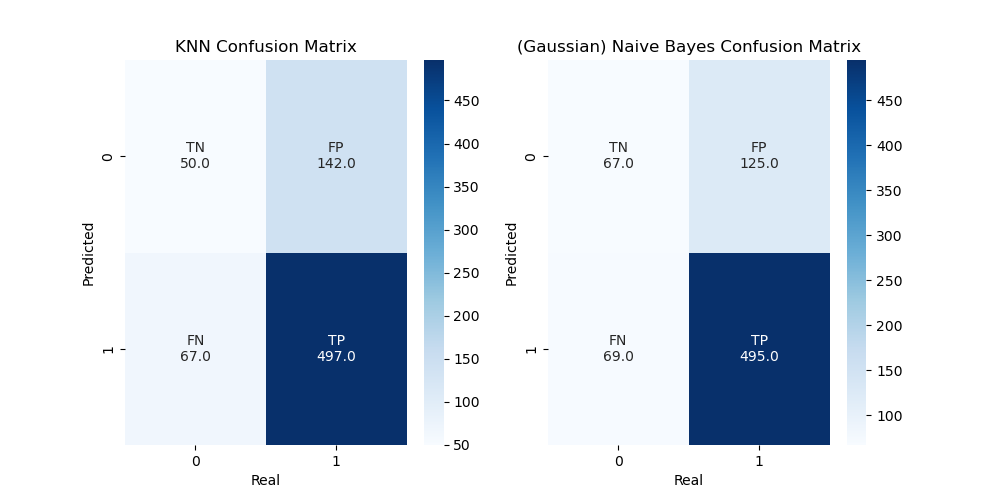
\includegraphics[width=1.1\textwidth]{../assets/hw2-2.1.png}
    \caption{Cumulative testing confusion matrices of $k$NN and Naïve Bayes}
    \label{fig:fig1}
  \end{figure}

  \pagebreak

  \item \textbf{Using \texttt{scipy}, test the hypothesis “$k$NN is statistically superior to Naïve Bayes regarding
  accuracy”, asserting whether is true.}

  \texttt{scipy.stats} provides the \texttt{ttest\_rel} function, which can be utilized
  to test a hypothesis given two related samples - here, both $kNN$'s and Naïve Bayes'
  scores are inherently related, since we're working with the same dataset on both
  classifiers, hence we can use this function to test the hypothesis.
  
  We opted to utilize it with a \texttt{alternative = 'greater'} parameter, since
  we're interested in testing whether $kNN$'s accuracy is statistically superior
  to Naïve Bayes' accuracy, and not the other way around - as such, a "right-tailed"
  test is more appropriate.
  The considered hypotheses are, therefore:

  \begin{itemize}
    \item $H_0$: $kNN$'s accuracy is statistically equal to Naïve Bayes'
    \item $H_1$: $kNN$'s accuracy is statistically superior to Naïve Bayes'
  \end{itemize}

  As a side-note, we've considered, in absence of a given confidence level in the
  question's statement, a confidence level of $1 - \alpha = 0.95$.
  After performing the test, we obtained a \textit{p-value} of $\approx 0.9104$ and
  a \textit{t-statistic} of $\approx -1.457$, which leads us to assert that, given
  $\alpha = 0.05$, we cannot reject the null hypothesis: we can't, therefore,
  assert whether $kNN$'s accuracy is statistically superior to Naïve Bayes'.
   
  \item \textbf{Enumerate three possible reasons that could underlie the observed differences in predictive
  accuracy between $k$NN and Naïve Bayes.}

  Note: the \href{https://fenix.tecnico.ulisboa.pt/disciplinas/Apre2/2022-2023/1-semestre/homeworks}{homework's FAQ}
  states that the answer could state as low as two reasons, even though the original
  question's statement states three. We opted to answer the question as stated in
  the FAQ.
  
\end{enumerate}

\pagebreak

\large{\textbf{Appendix}\vskip 0.3cm}

% The code utilized in the first question of the programming section is shown below:

% \lstinputlisting[language=Python]{code.py}

\end{document}
